\documentclass{beamer}
\usepackage[utf8]{inputenc}

\usetheme{Madrid}
\usecolortheme{default}
\usepackage{amsmath,amssymb,amsfonts,amsthm}
\usepackage{txfonts}
\usepackage{tkz-euclide}
\usepackage{listings}
\usepackage[T1]{fontenc}
\usepackage{adjustbox}
\usepackage{array}
\usepackage{tabularx}
\usepackage{gvv}
\usepackage{lmodern}
\usepackage{circuitikz}
\usepackage{tikz}
\usepackage{graphicx}

\setbeamertemplate{page number in head/foot}[totalframenumber]

\usepackage{tcolorbox}
\tcbuselibrary{minted,breakable,xparse,skins}

\definecolor{bg}{gray}{0.95}
\DeclareTCBListing{mintedbox}{O{}m!O{}}{%
  breakable=true,
  listing engine=minted,
  listing only,
  minted language=#2,
  minted style=default,
  minted options={%
    linenos,
    gobble=0,
    breaklines=true,
    breakafter=,,,,
    fontsize=\small,
    numbersep=8pt,
    #1},
  boxsep=0pt,
  left skip=0pt,
  right skip=0pt,
  left=25pt,
  right=0pt,
  top=3pt,
  bottom=3pt,
  arc=5pt,
  leftrule=0pt,
  rightrule=0pt,
  bottomrule=2pt,
  toprule=2pt,
  colback=bg,
  colframe=orange!70,
  enhanced,
  overlay={%
    \begin{tcbclipinterior}
    \fill[orange!20!white] (frame.south west) rectangle ([xshift=20pt]frame.north west);
    \end{tcbclipinterior}},
  #3,
}

\lstset{
    language=C,
    basicstyle=\ttfamily\small,
    keywordstyle=\color{blue},
    stringstyle=\color{orange},
    commentstyle=\color{green!60!black},
    numbers=left,
    numberstyle=\tiny\color{gray},
    breaklines=true,
    showstringspaces=false,
}

\title{4.8.10}
\author{AI25BTECH11014 - Gooty Suhas}

\begin{document}
\frame{\titlepage}

\begin{frame}{Question}
Find the foot of the perpendicular from
\[
\vec{P} = \myvec{3 \\ 2 \\ 1}
\]
to the plane
\[
\vec{N}^T \vec{x} = 1,\quad \vec{N} = \myvec{2 \\ -1 \\ 1}
\]
Also find the distance \( \|\vec{P} - \vec{Q}\| \) and the image of \( \vec{P} \) treating the plane as a mirror.
\end{frame}

\begin{frame}{Foot of Perpendicular}
We use:
\[
\vec{Q} = \vec{P} - \frac{\vec{N}^T \vec{P} - 1}{\vec{N}^T \vec{N}} \vec{N}
\]
Compute:
\[
\vec{N}^T \vec{P} = \myvec{2 & -1 & 1} \myvec{3 \\ 2 \\ 1} = 5
\quad \Rightarrow \quad \vec{N}^T \vec{P} - 1 = 4
\]
\[
\vec{N}^T \vec{N} = \myvec{2 & -1 & 1} \myvec{2 \\ -1 \\ 1} = 6
\Rightarrow \vec{Q} = \vec{P} - \frac{2}{3} \vec{N}
= \myvec{3 \\ 2 \\ 1} - \frac{2}{3} \myvec{2 \\ -1 \\ 1}
= \myvec{\frac{5}{3} \\ \frac{8}{3} \\ \frac{1}{3}}
\]
\end{frame}

\begin{frame}{Distance}
\[
\|\vec{P} - \vec{Q}\| = \left\| \frac{2}{3} \vec{N} \right\|
= \frac{2}{3} \sqrt{6}
\]
This is the perpendicular distance from \( \vec{P} \) to the plane.
\end{frame}

\begin{frame}{Image of \( \vec{P} \)}
The reflected image is:
\[
\vec{R} = \vec{P} - 2 \cdot \frac{\vec{N}^T \vec{P} - 1}{\vec{N}^T \vec{N}} \vec{N}
= \vec{P} - \frac{4}{3} \vec{N}
= \myvec{3 \\ 2 \\ 1} - \frac{4}{3} \myvec{2 \\ -1 \\ 1}
= \myvec{\frac{1}{3} \\ \frac{10}{3} \\ -\frac{1}{3}}
\]
\end{frame}

\begin{frame}{Final Answer}
\[
\boxed{
\vec{Q} = \myvec{\frac{5}{3} \\ \frac{8}{3} \\ \frac{1}{3}}
}
\quad
\boxed{
\|\vec{P} - \vec{Q}\| = \frac{2}{3} \sqrt{6}
}
\quad
\boxed{
\text{Image of } \vec{P}: \myvec{\frac{1}{3} \\ \frac{10}{3} \\ -\frac{1}{3}}
}
\]
\end{frame}


\begin{frame}[fragile]{Python Code — SymPy}
\begin{lstlisting}[language=Python]
from sympy import Matrix, sqrt

P = Matrix([3, 2, 1])
N = Matrix([2, -1, 1])

num = N.dot(P) - 1
den = N.dot(N)

Q = P - (num / den) * N
dist = (num / den) * sqrt(den)
R = P - 2 * (num / den) * N

print("Q =", Q)
print("Distance =", dist)
print("Image =", R)
\end{lstlisting}
\end{frame}



\begin{frame}[fragile]{C Code — Matrix Only (1/2)}
\begin{lstlisting}[language=C]
#include <stdio.h>
#include <math.h>

int main() {
    double P[3], N[3];
    for(int i = 0; i < 3; i++)
        scanf("%lf", &P[i]);
    for(int i = 0; i < 3; i++)
        scanf("%lf", &N[i]);

    double dotPN = 0, dotNN = 0;
    for(int i = 0; i < 3; i++) {
        dotPN += P[i] * N[i];
        dotNN += N[i] * N[i];
    }
\end{lstlisting}
\end{frame}


\begin{frame}[fragile]{C Code — Matrix Only (2/2)}
\begin{lstlisting}[language=C]
    double scalar = (dotPN - 1) / dotNN;
    double Q[3], R[3];
    for(int i = 0; i < 3; i++) {
        Q[i] = P[i] - scalar * N[i];
        R[i] = P[i] - 2 * scalar * N[i];
    }

    double dist = scalar * sqrt(dotNN);

    printf("Q = (%.3f, %.3f, %.3f)\n", Q[0], Q[1], Q[2]);
    printf("Distance = %.3f\n", dist);
    printf("Image = (%.3f, %.3f, %.3f)\n", R[0], R[1], R[2]);
    return 0;
}
\end{lstlisting}
\end{frame}


\begin{frame}[fragile]{Python Code — With .so}
\begin{lstlisting}[language=Python]
import subprocess

P = [3.0, 2.0, 1.0]
N = [2.0, -1.0, 1.0]
inputs = P + N
input_str = ' '.join(map(str, inputs))

result = subprocess.run(
    ['./plane_solver'],
    input=input_str,
    capture_output=True,
    text=True
)

print(result.stdout.strip())
\end{lstlisting}
\end{frame}










\begin{frame}{3D Plot}
\begin{figure}[H]
\centering
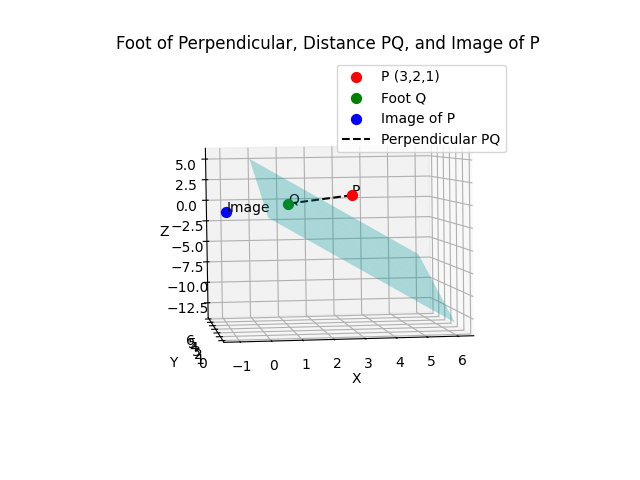
\includegraphics[width=1\linewidth]{Figs/Fig_1.png}
\caption{Foot of perpendicular \( \vec{Q} \), image of \( \vec{P} \), and plane \( \vec{N}^T \vec{x} = 1 \)}
\end{figure}
\end{frame}





\end{document}







